\title{CS3210 Assignment 1\\Particle Movement Simulator (Part 2)}
\author{Keven Loo Yuquan (A0183383Y) \& Lee Yong Jie, Richard (A0170235N)}
\date{}

\documentclass[12pt]{article}

% Margins
\usepackage[margin=2cm]{geometry}
% Math and symbols
\usepackage{amsmath}
\usepackage{amssymb}
% Syntax highlighting
\usepackage{minted}
% Inclusion of pictures
\usepackage{graphicx}
\graphicspath{{./reportAssets/}{./processedResults/}{./extraProcessedResults/}}
% Better looking underlines
\usepackage{soul}
\setuldepth{Parallel}
% Combine texttt & textbf
\usepackage{bold-extra}
% No paragraph indentations
\setlength{\parindent}{0pt}
% Merge rows of table
\usepackage{multirow}
% Fixed tables
\usepackage{tabularx}
% LaTeX is dumb at deciding where figures should go
\usepackage{float}

% \bf formats a chunk of text to both texttt and textbf
\newcommand{\bt}[1]{\texttt{\textbf{#1}}}
% Center-aligned column
\newcolumntype{C}{>{\centering\arraybackslash}X}

\begin{document}
\maketitle
\setcounter{tocdepth}{1}
\tableofcontents

\pagebreak
\section{Program Design}

The discrete particle simulation is implemented fully in C and OpenMP. The overall architecture of the simulator is summarised in the diagram below.

\begin{figure}[hb]
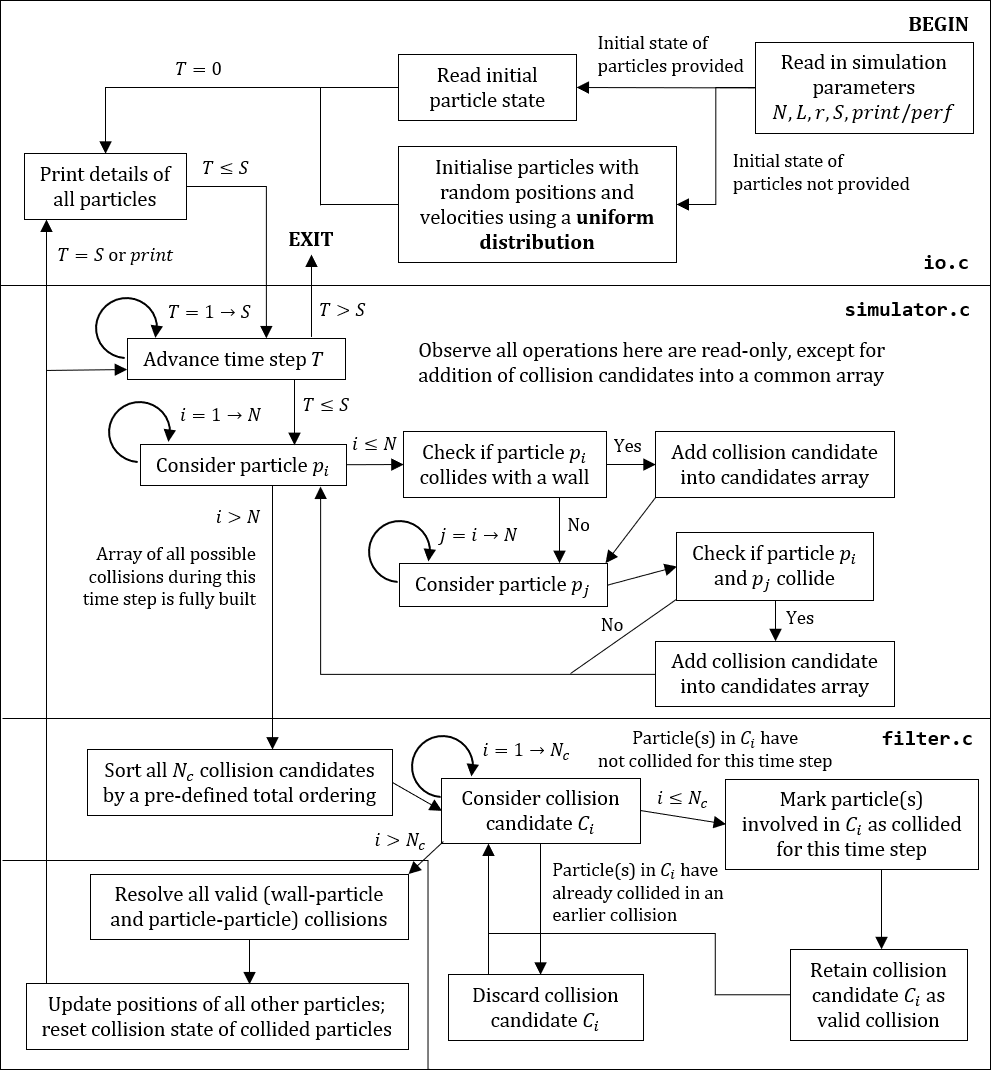
\includegraphics{chap1Flowchart}
\centering
\end{figure}

\pagebreak

\section{Implementation Assumptions and Details}

\subsection{Assumptions}

We make the following assumptions in our simulation.

\begin{enumerate}
	\item Even though the maximum initial velocity limit is $L/4$, we assume that the typical velocity of a particle is much less than this $\implies$ particles move only a small amount for each time step, hence for each particle $p_i$ and particle $p_j$, the probability of collision $P(p_i, p_j\ collide) \ll 1$ $\implies$ the total number of collisions per step $N_{collisions} = \Theta (N)$.
	\item A particle is involved in no more than one collision per time step.
	\begin{itemize}
		\item Implications
		\begin{enumerate}
			\item If a particle collides with a wall after any collision, it is placed at the wall at the end of that time step, ready to collide with the wall the next time step
			\item If particle $P$ collides with a particle $Q$ after any collision, it will phase through the particle $Q$ for the remainder of this time step, or will ignore $Q$ the next time step if they happen to overlap
		\end{enumerate}
	\end{itemize}
	\item All collisions between particles and with the wall are elastic (kinetic energy and momentum are conserved). 
	\item It is possible to fit all $N$ particles of radius $r$ into the square of length $L$ without overlapping.
	\begin{itemize}
		\item Implication
		\begin{enumerate}
			\item The simulation exits if one of these two conditions fail: $L < 2r$ (not possible to fit a single particle) or $Nr^2 > L^2$ (not possible to pack $N$ particles into a \ul{grid} in a square with area $L^2$)
		\end{enumerate}
	\end{itemize}
	\item The set of possible collisions $C$ satisfies a \textbf{total ordering}.
	\begin{itemize}
		\item Implication
		\begin{enumerate}
			\item For each time step $T$, it is possible to sort all collision candidates by this total ordering to determine which collisions should be prioritised over others.
		\end{enumerate}
	\end{itemize}
\end{enumerate}

\pagebreak

\subsection{Implementation Details}

\begin{enumerate}
	\item If the initial state of particles are not provided, particles are generated with initial random positions and velocities using a \textbf{uniform distribution}.
	\begin{enumerate}
		\item We use the pseudo-random number generator rand in the C library seeded with the number 3210.
		\item Particles are placed randomly in the square without overlapping.
	\end{enumerate}
	\item Each particle keeps track of its own state: $\textrm{ID}, x, y, v_x, v_y$.
	\item Our simulation has an additional parameter \texttt{SLOW\_FACTOR} in \texttt{simulator.c} that increases the granularity of the simulation for greater accuracy. \label{slow-factor-ref}
	\begin{enumerate}
		\item Setting \texttt{SLOW\_FACTOR} to an integer $>1$ slows the initial velocities of all particles by that factor. \texttt{SLOW\_FACTOR} should be set to a power of two to avoid introducing additional floating-point errors when dividing the particles’ velocities.
		\item The number of steps of the simulation is correspondingly multiplied by \texttt{SLOW\_FACTOR}, i.e. each original step now corresponds to \texttt{SLOW\_FACTOR} ``micro-steps".
	\end{enumerate}
	\item Collisions are of two types: either particle-wall collisions or particle-particle collisions. We describe a particle-wall collision as ($P$, \texttt{null}) and a particle-particle collision as ($P$, $Q$).
	\begin{enumerate}
		\item As particle-particle collisions are symmetric (i.e. $P$ collides with $Q$ $\iff$ $Q$ collides with $P$), we generate these collisions such that $P$ is the particle with lower integer ID.
	\end{enumerate}
	\item When sorting collision candidates with the C library function \texttt{qsort}, we enforce this total ordering in the function \texttt{cmpCollision}. For two collision candidates  $C_1$ and $C_2$,
	\begin{itemize}
		\item[$\blacksquare$] $C_1 < C_2$ if $C_1$ occurs before $C_2$
		\item[$\blacksquare$] If $C_1$ and $C_2$ occur at the same time
		\begin{itemize}
			\item[$\square$] $C_1 < C_2$ if the ID of $P$ in $C_1$ $<$ the ID of $P$ in $C_2$
			\item[$\square$] If $C_1$ and $C_2$ both involve the same particle $P$
				\begin{itemize}
					\item[$\blacksquare$] $C_1 < C_2$ if $C_1$ is a wall collision
					\item[$\blacksquare$] If $C_1$ and $C_2$ are both particle-particle collisions
						\begin{itemize}
							\item[$\square$] $C_1 < C_2$ if the ID of $Q$ in $C_1$ $<$ the ID of $Q$ in $C_2$
						\end{itemize}
				\end{itemize}
		\end{itemize}
	\end{itemize}
	\item For each particle in each time step, we check once if the particle collides with any of the four walls.
	\item (\textbf{Sequential and parallel-1}) All possible collision pairs are checked for each time step. The total number of collision checks performed is thus
	\begin{align*}
	N_{potential\ collisions} 	&= N_{wall-particle} + N_{particle-particle} \\
						&= N + \frac{N(N-1)}{2} \\
						&= \Theta (N^2)
	\end{align*}
	\item Particle-wall collisions are checked by solving the trajectory equation of a particle and the positions equations of the wall. The equations of the walls are $x = 0, x = L, y = 0, y = L$.
	\item \label{trajectory-calc} Particle-particle collisions are checked by solving trajectory equations of two particles during the given time step.
	
	Consider two particles $P$, $Q$ during a given time step $0 \leq \Delta t \leq 1$. From Pythagoras’ theorem, the distance between them is
	$$d = \sqrt{\left( \left( x_Q + v_{xQ} \Delta t \right) - \left( x_p + v_{xP} \Delta t \right) \right)^2 +
		\left( \left( y_Q + v_{yQ} \Delta t \right) - \left( y_p + v_{yP} \Delta t \right) \right)^2}$$
	or re-written in terms of deltas (differences in state)
	$$d = \sqrt{\left( \Delta x + \Delta v_x \Delta t \right)^2 +
		\left( \Delta y + \Delta v_y \Delta t \right)^2}$$
		
	The particles intersect when $d = 2r$, i.e. the particles touch at their circumference, hence by expanding and collecting terms we get the quadratic equation of form $A (\Delta t)^2 + B \Delta t + C = 0$,
	
	\begin{align*}
		\Delta x^2 + 2 \Delta x \Delta v_x \Delta t + \Delta v_x^2 (\Delta t)^2 + \Delta y^2 + 2 \Delta y \Delta v_y \Delta t + \Delta v_y^2 (\Delta t)^2 &= (2r)^2 \\
		\implies (\Delta v_x^2 + \Delta v_y^2) (\Delta t)^2 + (2 \Delta x \Delta v_x + 2 \Delta y \Delta v_y) \Delta t + (\Delta x^2 + \Delta y^2 - 4r^2) &= 0
	\end{align*}
	
	We observe that $A = (\Delta v_x^2 + \Delta v_y^2) > 0$ and thus the curve $y = d(\Delta t)$ is concave up. The discriminant for this quadratic equation, $B^2 - 4AC$, is
	$$\textrm{discriminant} = (2 \Delta x \Delta v_x + 2 \Delta y \Delta v_y)^2 - 4(\Delta v_x^2 + \Delta v_y^2)(\Delta x^2 + \Delta y^2 - 4r^2)$$
	
	If this discriminant is $\geq 0$, then the particles collide for some value of $\Delta t$, and we solve for this $\Delta t$. There are two possible roots,
	$$\Delta t = \frac{-B \pm \sqrt{\textrm{discriminant}}}{2A}$$
	
	Since the quadratic curve is concave up, we only compute and examine the first root (when the particles are approaching each other). This is
	$$\Delta t = \frac{-B - \sqrt{\textrm{discriminant}}}{2A}$$
	
	If $0 \leq \Delta t \leq 1$, then particles $P$, $Q$ collide during this time step.
	
	Note that, it is possible for $\Delta t < 0$ - this corresponds to cases where particles are overlapping from a previous step. We do not consider these as collisions in the current step and let these two particles phase through each other.
\end{enumerate} 

\pagebreak

\section{Parallelisation Strategy}

% TODO discussion
\subsection{Host-device distribution}

\subsection{Problem decomposition}

% \subsection{Floating-point inconsistencies}
% TODO does floating point inconsistencies get discussed here?
% shouldnt fall under parallelisation strategy..?

\pagebreak

\section{Test Conditions and Testcases}

\subsection{Test Setup}

% TODO: update test setup
% nodes used: xgpe1, xgpf0, jetsontx2-01, soctf-pdc-010 (20 threads)

Benchmarking of our sequential, parallel and early-pruning implementations were done on the same lab machines with aid of a Python script to generate input files (\texttt{generateTestcases.py}) and a Bash script to execute and log output for each testcase. These files can be found in the \texttt{<impl>BatchRuns} sub-folder of the respective implementation (under \texttt{/code/<impl>/}). \\ % TODO: 

The Intel i7-7700K node tested was \ul{soctf-pdc-001} and the Intel Xeon Silver 4114 node tested was \ul{soctf-pdc-010}. Each testcase was run five times and the fastest execution time was retained as the datapoint for that testcase. \\

To replicate our results for a given implementation, compile all files in that folder with \bt{gcc *.h} followed by \bt{gcc -fopenmp *.c -lm}. Then, execute the corresponding Bash script in the associated \texttt{<impl>BatchRuns} sub-folder. % update testing?

\subsection{Random Testcases}

% TODO: update random testcases
% N = 1000, 2000, 3000, 4000, 6000 (jetson + others)
% N = 8000, 12000, 16000, 24000, 32000 (others)
% L = 20000, r = 1, S = 1000

For benchmarking, testcases ran in \textit{perf} mode and the initial states of particles were not provided. Variables of the simulation were adjusted for each testcase. \\

The simulation parameters of the default testcase are
\begin{itemize}
	\item $N = 1000, L=20000, r=1, S=1000$
\end{itemize}

The testcases that were executed for each implementation are as follows. 
\begin{enumerate}
	\item Sequential implementation
	\begin{itemize}
		\item Varying $N$ only: $N = 250, 375, 500, 750, 1500, 2000$
		\item Varying $L$ only: $L = 5000, 7500, 15000, 20000$
		\item Varying $r$ only: $r = 1, 2, 3, 4, 6, 8, 16$
		\item Varying $S$ only: $S = 250, 375, 500, 750, 1500, 2000$
	\end{itemize}
	
	\item Parallel implementation
	\begin{itemize}
		\item $T$ = number of OpenMP threads
		\item Varying both $N$ and $T$ together
		\begin{itemize}
			\item $N = 250, 500, 1000, 2000$
			\item $T = 1, 2, 4, 6, 7, 8, 9, 10, 12, 16, 19, 20, 21, 24, 28, 32, 40, 64$
		\end{itemize}
	\end{itemize}
\end{enumerate}

\pagebreak

\subsection{Special Testcases}

% TODO: remove this section?

In addition to the random testcases, we designed a few additional special testcases to assert correctness of our simulator, alongside an extra Python script (in folder \texttt{/scripts}: \texttt{generateAnimation.py}) to visualise the simulation output. We provided the \texttt{.GIF} visualisations for each of these testcases. \\

Each of these testcases are named accordingly, and should be run with \texttt{SLOW\_FACTOR} set to a power of two (we recommend 16) for accuracy. Running these testcases with other values of \texttt{SLOW\_FACTOR} may lead to different results due to floating-point errors or insufficient granularity of simulation. \\

These testcases are as follows.

\begin{itemize}
	\item \texttt{cradle.in} - a horizontal row of particles that behaves like Newton’s cradle, endlessly bouncing between two walls
	\item \texttt{cross.in} - two particles bouncing between opposite diagonals of the square, without ever colliding
	\item \texttt{diagonalLine.in} - a diagonal row of particles bouncing from left to right, with glancing collisions
	\item \texttt{square.in} - four particles colliding at the same time at the centre; all four particles are deflected exactly at right angles from their initial trajectory
	\item \texttt{triangle.in} - three particles colliding at the same time, with resolution to prioritise the collision between the pair of particles with lowest ID
\end{itemize}

\pagebreak

\section{Execution Time Results}

All plots were generated with the help of R. The raw data from the \bt{perf stat} command is available in the submission as \texttt{.csv} files in \texttt{/data/sequential} and \texttt{/data/sequentialVsParallel}. Some of the plots are not reproduced here for brevity. % TODO: To update filepaths

% TODO: add plots here

\pagebreak

\section{Discussion: GPU Implementation}

% TODO: discussion here

\subsection{Execution time and speedup}

\subsection{Difference in devices}

\end{document}
